\documentclass{ees}

\newgeometry{twoside=false,left=20mm,right=40mm,top=20mm,bottom=40mm}

\newlist{bulletlist}{itemize}{1}
\setlist[bulletlist]{
  partopsep=0pt,
  parsep=0pt,
  itemsep=0pt,
  label=\textbullet
}

\setcounter{tocdepth}{1}
\DeclareTOCStyleEntry[
  indent=0pt,
  beforeskip=\baselineskip,
  entrynumberformat=\@gobble,
  entryformat=\sbseries,
  numwidth=2em,
  linefill=\hfill,
  pagenumberbox=\pnumbox,
  pagenumberformat=\sbseries
]{tocline}{chapter}


\begin{document}

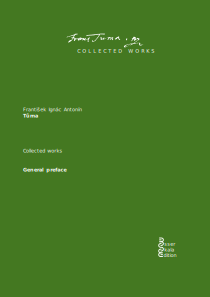
\includepdf{cover_general_preface.pdf}
\pagenumbering{arabic}
\setcounter{page}{1}

\tableofcontents

\chapter{General preface}

\textit{František Ignác Antonín Tůma: Collected works} (FIAT:CW) is an edition project that will make Tůma’s music available in modern editions.

For detailed information on Tůma's works, we refer the reader to our thematic catalogue of works (\href{https://www.frantisek-tuma.at/}{https://www.frantisek-tuma.at/}), which is currently under development. TumW numbers are cited from this catalogue.


\section{Editorial guidelines}

In general, FIAT:CW follows the \href{https://edition.esser-skala.at/about/editorial-guidelines/}{editorial guidelines} for the Edition Esser-Skala.

% Some peculiarities for editing Tůma's works are highlighted below:

% \begin{bulletlist}
%   \item
% \end{bulletlist}


\section{Acknowledgements}

Assistance of the following people and institutions is gratefully acknowledged:
Thomas Dolezal (Dommusikarchiv Eisenstadt – A-Ed),
Ute-Eva Thiem (Benediktinerabtei Stift Göttweig, Musikarchiv – A-GÖ),
P. Roman Nägele (Stift Heiligenkreuz im Wienerwald, Musikarchiv – A-HE),
P. Altman Pötsch (Benediktinerstift Kremsmünster, Regenterei und Musikarchiv – A-KR),
Peter Deinhammer (Benediktinerstift Lambach, Musikarchiv – A-LA),
Christian Schüller (Röm.-Kath. Pfarramt Maria Taferl – A-MT),
Ikarus Kaiser (Stift Wilhering, Musikarchiv – A-WIL),
Ludmila Šmídová (Národní knihovna České republiky, Praha – CZ-Pu),
Christian Filips (Sing-Akademie zu Berlin, Notenarchiv – D-Bsa),
Martin Lang (Bistum Passau, Archiv – D-Po),
Damásdi Zoltán (Pécsi Egyházmegye, Pécsi Püspöki Levéltár, Székesegyházi Kottatár – H-P),
Alessia Ravagnani (Museo internazionale e biblioteca della musica di Bologna – I-Bc),
Sebastian Lindblom (Musik- och teaterbiblioteket, Stockholm – S-Skma),
as well as the staff of
the Österreichische Nationalbibliothek, Musiksammlung, Wien (A-Wn),
the Staatsbibliothek zu Berlin - Preußischer Kulturbesitz, Musikabteilung (D-B),
the Universität der Künste Berlin, Universitätsbibliothek, Berlin (D-Bhm),
the Sächsische Landesbibliothek - Staats- und Universitätsbibliothek, Dresden (D-Dl),
the Badische Landesbibliothek, Musiksammlung, Karlsruhe (D-KA),
and the Universitetsbiblioteket Lund (S-L).


\clearpage
\markdownInput{../CHANGELOG.md}

\end{document}
